\documentclass[output=paper,
modfonts
]{langscibook} 

\title{A morpho-semantic account of weak definites and bare institutional singulars in English} 

\shorttitlerunninghead{A morpho-semantic account of weak definites and bare institutional singulars}

\author{%
 Adina Williams\affiliation{New York University}}

% \chapterDOI{} %will be filled in at production
% \epigram{}

\abstract{
Weak definites in \ili{English} have been widely studied as an example of when the \is{definite articles}definite article doesn't contribute \isi{uniqueness} (\citealt{Aguilar-GuevaraZwarsts2011,Aguilar-GuevaraEtAlii2014}, among others). I take \textit{uniqueness} to stem from the interaction between definiteness and \isi{number} within the \is{noun phrases}noun phrase. From this perspective, weak definites should be seen as a data point situated in the larger cross-literature on number. One particular phenomenon from the literature on number, the understudied class of the \ili{English} bare institutional singulars (BISs), has been discovered to share several semantic properties with \isi{weak definiteness}, namely \isi{number neutrality}, referential deficiency, and lexical idiosyncrasy. In this chapter, I postulate a shared account of \ili{English} weak definites and BISs that utilizes \isi{semantic root ambiguity} \citep{RappaportLevin1998,Levinson2014} as a way to account for these facts. This account has syntactic consequences that resonate with recent \is{morphosyntax}morphosyntactic accounts of number phenomena that argue {Num}P is the host of number interpretation and marking \citep{ritter1991,ritter1992,ritter1995} in languages like Amharic\il{Amharic}, \citep{Kramer2009}, \il{Salish!Halkomelem Salish}Halkomelem Salish \citep{wiltschko2008}, and \ili{Haitian Creole} \citep{Deprez2005}. 
}

\shorttitlerunninghead{A morpho-semantic account of weak definites and BISs}

\begin{document}
\maketitle

\section{Introduction}\label{sec:williams:1}\is{morphosemantics|(}\is{number neutrality|(}\is{bare institutional singulars|(}\is{weak definites|(}

Noun phrase constructions called \textit{weak definites} \citep{BirnerWard1994,Poesio1994} have been heavily studied in \ili{English} \citep{CarlsonSussman2005,CarlsonEtAlii2006,Aguilar-GuevaraZwarsts2011,Aguilar-Guevara2014} and other languages \citep{Schwarz2009,Schwarz2013,Schwarz2014}. They pose a problem for classical accounts of \isi{definite noun phrases} \citep{Frege1892,Russell1905,Hawkins1978,Sharvy1980,Heim1982} which require them to be referential and denote \is{uniqueness|(}unique individuals in the \isi{discourse}, as is evidenced by \REF{ex:williams:1} below. 

\begin{exe}\il{English}
	\ex{\label{ex:williams:1}
		\textit{Bob went to \textbf{the store} and Mary did too.} \citep[19]{Carlson2006b} \\ (Different stores OK.)}
	\ex{\label{ex:williams:2}
		\textit{Bob is in \textbf{jail} and Fred is too.} \citep[18]{Carlson2006b} \\ (Different jails OK.)}
\end{exe}

Interestingly, \ili{English} has yet another \is{noun phrases}noun phrase construction -- the \textsc{bare institutional singular} (BIS), as in \REF{ex:williams:2} -- that is not \is{definiteness marking} marked for definiteness, but shares many semantic properties with the weak definite, including number neutrality, diminished referential capacity, and lexical idiosyncrasy. Although it has been noted that not all lexical items can participate in weak definite and BIS constructions \citep{Carlson2006b,CarlsonEtAlii2006,Aguilar-GuevaraZwarsts2011,Aguilar-GuevaraEtAlii2014,Aguilar-GuevaraSchulpen2014}, very few accounts have used this fact as fundamental in their analysis of weak definites \citep[but see][]{BaldwinEtAlii2006}. In this chapter, I propose a shared account for both weak definite and BIS constructions that accounts for both their interpretive similarities and their lexical idiosyncrasy. 

I propose that interpretive similarities between weak definite and BIS constructions can be derived via \is{semantic root ambiguity}root semantic type ambiguity \citep[see][]{RappaportLevin1998}, parallel to \citet{Levinson2014} on verbal argument structure alternations. The lexical items that can occur in weak definite or BIS constructions have a many-to-one mapping between their syntactic roots and potential denotations of those roots, unlike most lexical items (e.g. the \is{strong definites|(}\textit{strong definites}\footnote{I use the term \is{strong definites}\textit{strong} to mean definites that are unique and referring, which is slightly different from the use of the term in \citet{Schwarz2009,Schwarz2013}.}) that have a one-to-one mapping. Interestingly, no lexical item can participate in both weak definite and BIS constructions, suggesting that, although roots from both classes are special in that they are semantically ambiguous, the two subclasses of roots are associated with different pairs of possible denotations. Furthermore, the root denotation interacts with whether a definite \is{determiners}determiner can be merged later in the derivation, and determines which of two versions of the determiner can be merged.\newpage

I restrict my focus to weak nominal constructions\footnote{The term \textit{weak definite} does not necessarily correspond to a single, uniform class in either the syntactic or semantic sense, and thus, different subtypes of weak definites have been given a wide range of theoretical and \is{experimental study}experimental treatments (see, for example, \citealt{Barker2005,KleinEtAlii2009,Aguilar-GuevaraZwarsts2011,Klein2011,Aguilar-GuevaraSchulpen2014,Schwarz2014}), and extending this account to other subtypes (e.g. those given in \citealt{stvan1998}) is left for future work.} utilizing directional predicates with location/institution \isi{nouns}, because they provide a unique testing ground for investigating the relationship between \isi{number} and definiteness. Representative sentences of the three types are given below in (\ref{ex:williams:3}--\ref{ex:williams:5}):

\begin{exe}\il{English}
	\ex{\label{ex:williams:3}
		\textit{Ron went to \textbf{the store}}. \hspace{2.8em} \textsc{weak definite singular} }
	\ex{\label{ex:williams:4}
		\textit{Ron went to \textbf{school}}. \hspace{3.95em} \textsc{bare institutional singular}}
	\ex{\label{ex:williams:5}
		\textit{Ron went to \textbf{the castle}}.\hspace{2.69em} \is{strong definites}\textsc{strong definite singular} }
\end{exe}

In my examples, I hold the main verb and \is{prepositions}preposition constant, because altering either has been shown to affect the availability of the number neutral interpretation \citep[18--19]{Aguilar-Guevara2014}. Although other verbal predicates can be used in sentences that get weak readings, I use the light verb \textit{to go} because it is compatible with all three sentence types (\ref{ex:williams:3}--\ref{ex:williams:5}). Because of their restricted syntactic distribution, weak definites are often cited as having an ``idiomatic'' flavor \citep{NunbergEtAlii1994} -- a property they share with BISs. I chose to use lexical items from the location/institution class of weak definites \citep{stvan1998} and BISs, because they are the most freely combining \citep{BaldwinEtAlii2006}, making them a good class to work with.  

This chapter is organized as follows. \sectref{sec:williams:2} argues in favor of interpretive similarities between weak definites and BISs. \sectref{sec:williams:3} discusses the lexical idiosyncrasy of roots that participate in weak definite and BIS constructions. \sectref{sec:williams:4} discusses syntactic consequences of adopting a \is{semantic root ambiguity}root semantic type ambiguity account of weakness in \ili{English} nominals. \sectref{sec:williams:5} provides a \is{morphosyntax}morpho-syntactic analysis that builds on work on cross-linguistic \isi{number} that suggests number neutrality has a syntactic reflex, i.e. a lack of a Num projection (as in languages with \textit{general number}). I also show that the denotation of roots affects which interpretations and syntactic structures are possible. Finally, \sectref{sec:williams:6} concludes.\is{number neutrality|)}

\section{Weak definite singulars and bare institutional singulars share semantic properties}\label{sec:williams:2}

Weak definite singulars and BISs share interpretive similarities with each other, to the exclusion of strong, referring definite singulars. There are multiple diagnostics for weakness \citep[see][]{CarlsonSussman2005}, all of which indicate that BISs and weak definites do not have to refer to a singular entity: they can be used in contexts where multiple entities can satisfy the descriptive content of the \is{definites}definite, they can receive \isi{sloppy identity} under \isi{VP ellipsis}, their behavior differs from that of referring definites under a type of sluice (under a novel diagnostic test), and they have an impaired ability to antecede pronouns in the following \is{discourse}discourse. 

Before I present the diagnostic tests, it is important to caution the reader that some weak definite Det-N strings are ambiguous between weak and strong interpretations. Therefore, I use a subset of lexical items for each class of nominals to help readers access the appropriate readings throughout this section (these lexical items are provided in the footnotes to \tabref{tab:williams:1} for reference). 

\begin{table}[h]\is{definiteness marking}
\caption{Classes of lexical items}
\label{tab:williams:1}
\begin{tabularx}{\textwidth}{llll} 
 \lsptoprule
            & +Definite marked & -Definite marked \\ 
 \midrule
 Weak interpretation  &   \textsc{weak definite}\footnote{Relevant lexical items: e.g.  \textit{the store, the bank, the hospital} (potentially ambiguous between weak and strong definite interpretations).} &     \textsc{bare institutional singular}\footnote{Relevant lexical items: e.g. \textit{school, church, prison, jail} (unambiguously weak).}      \\
 Strong interpretation  &   \textsc{strong definite}\footnote{Relevant lexical items: e.g. \textit{the castle, the stadium, the restaurant} (unambiguously strong).}  &  *\footnote{I assume this cell is empty due to the \is{Blocking Principle}Blocking Principle discussed in \citet[360]{Chierchia1998}, and \citet{DealNee2016}. The Blocking Principle states that \isi{bare nominals} cannot be interpreted as definite, because there is a lexically specified \is{type shifting}type shifter present in the language that performs this function.}   \\
 \lspbottomrule
\end{tabularx}
\end{table}

\subsection{Multiple entities satisfying descriptive content}\label{sec:williams:2.1}

Weak definites and BISs can be used in contexts where multiple entities satisfy the descriptive content of the \is{noun phrases}noun phrase, suggesting that they don't uniquely refer \citep{CarlsonSussman2005}. In (\ref{ex:williams:6}--\ref{ex:williams:8}) below, each of the bolded noun phrases fails to require a single unique referent: 

 \begin{exe}\il{English}
 	\ex{\label{ex:williams:6}
 		\textit{Don went to \textbf{the zoo}.}}
 	\ex{\label{ex:williams:7}
 		\textit{Sue took her nephew to \textbf{the hospital}/\textbf{the store}/\textbf{the beach}.} \citep[2]{CarlsonEtAlii2006}}
 	\ex{\label{ex:williams:8} 
 		\textit{Please take \textbf{the elevator} to the second floor.} \citep[14]{Aguilar-Guevara2014}}
 \end{exe}
 
Although the examples above can be used to refer to identifiable, unique referents in the \isi{discourse}, one can also utter \REF{ex:williams:6} in cities where there are multiple zoos, \REF{ex:williams:7} in towns where there are multiple hospitals, stores or beaches, and \REF{ex:williams:8} when standing before a bay of elevators. Furthermore, weak definites can also be used in situations with multiple potential referents in the discourse, allowing the weak definite noun phrase to stand for a plurality of entities:\footnote{The interpretation of the following examples is not exhaustive; they are infelicitious in situations where there are only e.g. four stores, as in \REF{ex:williams:9}.}

\begin{exe}\il{English}
	\ex{\label{ex:williams:9}
	Context: Ron has been looking for Don, who was supposed to help him set up a party, but then went missing for a while.\\
    Ron: \textit{Hey Don! Where have you been? The party starts in an hour!}\\
    Don: \textit{I went to \textbf{the store} to buy balloons. I had to go to \textbf{four of them} because the first three were all sold out!}}
\end{exe}

In the mini-discourse in \REF{ex:williams:9}, the bolded \is{definiteness marking}definite marked noun phrase \textit{the store} does not impose a restriction that there only be a single, unique store in the context, because immediately following the \is{definites}definite, Don mentions that he went to \textit{four of them}. If the \is{definite noun phrases}definite noun phrase in \REF{ex:williams:9} did impose this restriction, we would predict the mini-discourse to be infelicitious. Similarly, the \is{bare singulars}bare singular, as in \REF{ex:williams:10}, can also be used felicitiously in situations where multiple entities satisfy the BIS's descriptive content. 

\begin{exe}\il{English}
	\ex{\label{ex:williams:10}
	Context: Ron just met up with Don at their ten-year high school reunion.\\
    Ron: \textit{Hey Don! Wow, you look great! What have you been up to for the last ten years?}\\
    Don: \textit{Funny you should ask... Actually I went to \textbf{prison} for five years after high school. I spent the first three years on Riker's Island, and the last two, in Alcatraz.}}
\end{exe}

Since BISs and singular weak definite noun phrases both lack the \isi{uniqueness} required for strong definite descriptions under this diagnostic, one would hope that the two types of weak nominal should have some grammatical similarities. Compare the two discourses above with the one below:

\begin{exe}\il{English}
	\ex{\label{ex:williams:11}
	Context: Ron and Don are on a vacation in Britain. They split up for a few days and are just meeting up again to continue on their adventure. The two had discussed their travel plans before splitting up.\\
    Ron: \textit{Hey Don! How did your weekend go? See anything interesting?}\\
    Don: \textit{Yeah, I had a really great weekend. I went to \textbf{the castle} and got some great pictures. \textnormal{??}On Saturday, I went to Windsor Castle, then took a train over to Dover Castle on Sunday.}}
\end{exe}

In this case, because Don's response is unnatural, I conclude that the \is{definite noun phrases}definite noun phrase \textit{the castle} requires a single, unique referent in the \isi{discourse}. The incompatibility of \REF{ex:williams:11} suggests that the lexical item conditions whether the \isi{uniqueness} presupposition is present, since it is unacceptable to use the singular definite noun phrase \textit{the castle} in a context where there are multiple castles.

\subsection{Sloppy readings under VP ellipsis}\label{sec:williams:2.2}\is{sloppy identity|(}\is{VP ellipsis|(} 
Singular weak definites and BISs differ from strong definites in that they do not require that the elided noun and the overt one refer to the same exact individual; they merely require that the individual(s) they refer to satisfy the descriptive content of their shared noun phrase. This loose identity requirement on \isi{noun phrases} under VP ellipsis is called \textsc{sloppy identity}. 

\begin{exe}\il{English}
	\ex{\label{ex:williams:12}
		\textit{Bob went to \textbf{the store} and Mary did too.} \citep[19]{Carlson2006b} \\(Different stores OK.)}
	\ex{\label{ex:williams:13}
		\textit{Bob is in \textbf{jail} and Fred is too.} \citep[18]{Carlson2006b}\\ (Different jails OK.)} 
\end{exe}

If the noun phrases in the antecedent VP in \REF{ex:williams:12} and \REF{ex:williams:13} are still faithfully duplicated in the ellipsis site, then presumably they cannot be strong definite noun phrases. Under VP ellipsis, they only need to match in the syntactic material that is present. Since the syntactic material present does not introduce a unique noun phrase, strict coreference is not required. In other cases, the \is{nouns}noun in the elided phrase is required to be coreferential with the \is{uniqueness|)}unique singular individual in the antecedent VP, as in \REF{ex:williams:14}:

\begin{exe}\il{English}
	\ex \label{ex:williams:14}
		\textit{Ron went to \textbf{the castle} and Don did too.} \jambox[0pt]{(strong reading only)}  
		\leavevmode 
		(Must be the same castle.) 
\end{exe}

In \REF{ex:williams:14}, there is a full \is{strong definites}strong noun phrase present in the ellipsis site. We only get a felicitious interpretation if the overt noun phrase and elided one refer to the same individual. In \REF{ex:williams:15} below, we can see that \textit{the store} is interpreted as a weak definite based on this diagnostic from above: 

\begin{exe}\il{English}
	 \ex{\label{ex:williams:15}
	 	\textit{Ron went to \textbf{the store} and Don did too. Ron went to Krogers, and Don went to Meijers.}}
\end{exe}

We can see that \textit{the store} in \REF{ex:williams:15} can be used felicitiously in VP ellipsis contexts, where multiple locations satisfy the descriptive content of the \is{noun phrases}noun phrase.\is{sloppy identity|)}\is{VP ellipsis|)}

\subsection{Sluicing}\label{sec:williams:2.3}\is{sluicing}

One final diagnostic, which is novel, comes from another ellipsis phenomenon, sluicing \citep{ross1967,ross1969}. Sluicing separates strong definites from weak definites and BISs, as the latter two are acceptable under a sluice, and the former is not:

\begin{exe}\il{English}
   	\ex{\label{ex:williams:16}
   		\textit{I know Ron went to \textbf{church} as a kid, but I don't know which one/church.}} 
 	\ex{\label{ex:wlliams:17}
 		\textit{I know Don went to \textbf{the store} after work, but I don't know which one/store.}} 
	\ex[??]{\label{ex:williams:18}
		\textit{I know Don went to \textbf{the castle} after work, but I don't know which one/cas\hyp{}tle.}}
\end{exe}

In \REF{ex:williams:18}, one must have a referent in mind to felicitiously use the \is{definiteness marking}definite marked noun phrase, which explains the unnaturalness of the sluice. Since \REF{ex:williams:16} and \REF{ex:wlliams:17} are acceptable under the sluice, one particular referent is not required. Thus, like the ellipsis diagnostic above in \sectref{sec:williams:2.3}, sluicing allows us to argue for the lack of referentiality present in weak nominals. 


\subsection{Limited capacity to establish discourse referents}\label{sec:williams:2.4} 

Following \citet[182]{Aguilar-GuevaraZwarsts2011}, I note that weak definites and BISs have a limited ability to establish \is{discourse}discourse referents, which results in them being  worse than strong definites at anteceding pronominal \textit{it}. I assume that anaphorically linked noun phrases, like \textit{it}, must match their antecedent in as many features (such as \isi{number} specification and referentiality) as possible. If \textit{it} is taken to be (generally) referring, and specified for singular, then it will have trouble matching its features with weak nominals that are neither referring nor specified as being singular (see \sectref{sec:williams:2.1}). If there is only one nominal in the context, and it is referential and singular, \textit{it} can be anaphorically linked to it, as in \REF{ex:williams:19} and \REF{ex:williams:20}:

\begin{exe}\il{English} 
	\ex{\label{ex:williams:19}
		\textit{Ron went to \textbf{the store} and Don went to \textbf{it} too. They both went to Krogers.}}
	\ex{\label{ex:williams:20}
		\textit{Ron went to \textbf{the castle} and Don went to \textbf{it} too. They both went to Neu\-schwanstein Castle.}}
\end{exe}

However, if we have pronominal \textit{it} -- which is referring (in this case), and wants to match its \isi{number} features with its antecedent -- in a context with multiple potential referents (as in \ref{ex:williams:21}), the sentence becomes less felicitious.

\begin{exe}\il{English}
 	\ex{\label{ex:williams:21}
 		\textit{Ron went to \textbf{the store} and Don went to \textbf{it} too. \textnormal{?}Ron went to Krogers, and Don went to Meijers.}}
\end{exe}    

Despite the fact that lexical items like \textit{store} can participate in weak definite constructions, by establishing coreference with \textit{it} in \REF{ex:williams:21}, the \is{noun phrases}noun phrase \textit{the store} can only receive a strong, referring interpretation. One way to encode this difference would be to say that some singular definite noun phrases (like \textit{the store}) are actually ambiguous between noun phrases that are un-marked for number, and those that are marked for singular. In \ili{English}, these two options will be string identical. When a pronoun tries to establish coreference with a \is{definite noun phrases}definite noun phrase that is un-marked for number, the result is degraded, as in \REF{ex:williams:21}.

If pronouns must match features with their antecedents, non-referring noun phrases like BISs should not have enough features to match with the pronoun, and thus should be even more degraded. This prediction is borne out:

\begin{exe}
 	\ex{\label{ex:williams:22}
 		\textit{Don went to \textbf{church}}\textsubscript{i} \textit{and Ron went to \textbf{it}}\textsubscript{*i,j} \textit{too.}}
\end{exe}

Establishing an \is{anaphora}anaphoric link with a referring pronoun is less acceptable for weak definites, but the BISs are unable to establish coreference with the pronoun at all. Therefore, one could assume that there are two missing features that make BISs unable to set up coreference, while for weak definites, there is only one (i.e. the number feature is missing). I claim that {Num}P is the crucial projection that is missing in both types of weak nominals; see \sectref{sec:williams:4} for further discussion.


\subsection{Summary}

In this section, I described the interpretive similarities that weak definites and BISs share to the exclusion of \isi{strong definites}; weak nominals can be used in situations where multiple entities satisfy the descriptive content (\sectref{sec:williams:2.1}), can receive \is{sloppy identity}sloppy readings under \isi{VP ellipsis} (\sectref{sec:williams:2.3}), are compatible with \isi{sluicing} (\sectref{sec:williams:2.3}), and have limited capacity to establish \is{discourse}discourse referents (\sectref{sec:williams:2.4}).\is{strong definites|)}

\section{Lexical idiosyncrasy}\label{sec:williams:3}

As discussed in the introduction, not all lexical items are equally able to participate in  weak constructions (see \tabref{tab:williams:1}). Weak definite and BIS interpretations are particularly sensitive to the identity of the lexical item:

 \begin{exe}
	\ex{\label{ex:williams:23}
		\textit{Don went to \textbf{the zoo}/\textnormal{\#}\textbf{the conservatory}.}} 
    \ex{\label{ex:williams:24}
    	\textit{Please take \textbf{the elevator}/\textnormal{\#}\textbf{the forklift} to the second floor.}}
    \ex{\label{ex:williams:25}
    	\textit{Sue took her nephew to \textbf{the hospital}/\textnormal{\#}\textbf{the hospice}.}}
\end{exe}

Even roots with comparable meanings (e.g. \textit{hospital} and \textit{hospice}) are unable to receive weak interpretations. It has been widely noted that weak interpretations for nominals are only available for certain lexical items, but few works other than \citet{BaldwinEtAlii2006} discuss this explicitly. Certain lexical items, e.g. \textit{store}, from the \textsc{weak-strong ambiguous} class can be interpreted as weak or as strong, while others, e.g. \textit{castle}, from the \textsc{strong-only} class can never be interpreted weakly (repeated from above, \ref{ex:williams:12} and \ref{ex:williams:14}). 

\begin{exe}
   	\ex{\label{ex:williams:26}
   		\textit{Ron went to \textbf{the store} and Don did too.} \\ (Can be the same store.)}
	\ex{\label{ex:williams:27}
		\textit{Ron went to \textbf{the castle} and Don did too.} \\ 
		(Must be the same castle.)}
\end{exe}

Because root identity seems to condition whether the weak reading is available, perhaps a \is{semantic root ambiguity|(}lexical ambiguity is present. This could mean that there are two denotations paired with the root, \textit{store}, but only one denotation for the root, \textit{castle}. I argue that this lexical ambiguity manifests itself in the semantic type of the root (a l\'a \citealt{Levinson2014}), as opposed to being a restriction on the type of elements that are present in the extension of the \is{noun phrases}noun phrase. 

The choice of root has consequences for the syntax. One piece of evidence in favor of a root-level semantic ambiguity that affects syntax is that the weak interpretation disappears when the root appears outside of constrained syntactic frames compatible with the weak interpretation. For example, \textit{store} cannot be interpreted weakly in subject position:\footnote{If the \is{nouns}noun is present in the subject position of a ``characterizing sentence'' in the sense of \citet{Carlson1977} and subsequent work, the \is{definite noun phrases}definite noun phrase can receive a \is{kinds}kind interpretation: 
\begin{exe} 
\exi{\fts{(i)}}
\textit{\textbf{The store} is a miraculous and entertaining place to visit.}
\end{exe} 
I take \is{kind reference}kind-referring noun phrases to be constructed differently than the definites I account for here, and leave an account comparing the two for future work.}

\begin{exe}
	\ex{\label{ex:williams:28}
		\textit{\textbf{The store} is closed today {\op}\textnormal{*}but I don't know which{\cp}.} \\
	{(Must be a strong reading.)} }
\end{exe}

Similarly, lexical items from the BIS class cannot receive a weak interpretation in subject position, see \REF{ex:williams:29}. However, when they occur with a \is{definite articles}definite article, they must receive a strong, referring interpretation; the weak interpretation is not allowed, see \REF{ex:williams:30}:

\begin{exe}
	\ex{\label{ex:williams:29}
		\textit{\textbf{School} is closed today.} \\ 
		(`School' here is a \is{proper names}proper name referring to the speaker's school, or to the \is{maximality}maximal set of all relevant schools.)} 
    \ex{\label{ex:williams:30}
    	\textit{Ron went to \textbf{the school} and Don did too.} \\ (Must be the same school.)}
\end{exe}

Thus, lexical items from each of the three classes can receive a referring interpretation when they are in \is{definiteness marking}\is{definite noun phrases}definite marked noun phrases, but only a subset can receive a weak interpretation when definite marked or \is{bare nominals}bare. Some roots can only receive strong interpretations (\textsc{strong only}). Some (roots from the \textsc{weak-strong ambiguous} class) can receive either. Yet, a third class of lexical items can be unmarked for plurality or definiteness, and also when they have definite marking, they can only receive a strong interpretation (\textsc{BIS}). The behavior of these classes of roots is summarized in \tabref{tab:williams:3}.\footnote{A lexical item that cannot get a strong or a weak interpretation, and cannot be \is{bare nominals}bare, is unlikely to exist. What would be its distribution? Would it only be present in \is{indefinites}indefinite noun phrases with \textit{a}? This doesn't seem very plausible. I leave the task of extending my lexical account to \isi{indefinites} to future work.} 

\begin{table}[h]\is{incorporation}\is{bare nominals}
\caption{Three lexical classes of roots}
\label{tab:williams:3}
\begin{tabularx}{\textwidth}{lccc} 
 \lsptoprule
 & \textsc{strong only} & \textsc{strong-weak ambig.}  & \textsc{bis}\\ 
 \midrule
 \textit{the}+NP can be strong  &  \textsc{Y} &     \textsc{Y}  &  \textsc{Y}  \\
 \textit{the}+NP can be weak  &   \textsc{N}  & \textsc{Y} & \textsc{N} \\
 can be bare/incorporated  &   \textsc{N}  & \textsc{N} & \textsc{Y} \\
 \lspbottomrule
\end{tabularx}
\end{table}

\subsection{Root semantic type ambiguity is not homophony}

I've argued that weakness starts at the root as a type difference, which then percolates up to affect higher syntactic projections. However, what sort of semantic ambiguity do we have in this case? I argue that this is a case of true ambiguity, and not simple homophony.  Under a homophony account, the roots have no inherent connection to each other. This would mean that we would have two lexical items that are both pronounced, e.g. \textit{store}, and that their interpretive similarity is accidental. 

One way to test for homophony was put forth in the general \isi{number} literature \citep{RullmannYou2006,wilhelm2008}. In this diagnostic, homophonous lexical items receive parallel interpretations under \isi{VP ellipsis}. I assume the following denotations\footnote{Type conventions are as follows: $x$, $y$, $z$ are from the domain of individuals and are type $e$; $e'$, $e''$, $e'''$ are from the domain of events and are type $v$; $m$, $n$ are from the domain of \is{number}numbers and are type $n$; $j$, $k$ are from the domain of kinds and are type $k$; type $t$ is for truth values; types can be combinatory; $P$, $Q$ are used for higher types, and their types are specified via subscript.} for the two homophonous lexical items: 

\begin{exe}
	\ex {\label{ex:williams:31}[\![pen\textsubscript{enclosure}]\!] :=$\lambda x. pen_{enclosure}(x)$}
	\ex {\label{ex:williams:32}[\![pen\textsubscript{implement}]\!] :=$\lambda x. pen_{implement}(x)$}
\end{exe}

\begin{exe}
	\ex \label{ex:williams:33}
	\textit{Lee saw a pen, and Sam did, too.}
	\begin{xlist}
		\ex[]{\label{ex:williams:33a}
			\textit{Lee saw an animal enclosure and Sam saw an animal enclosure too.}}
		\ex[]{\label{ex:williams:33b}
			\textit{Lee saw a writing implement and Sam saw a writing implement too.}}
		\ex[*]{\label{ex:williams:33c}
			\textit{Lee saw a writing implement and Sam saw an animal enclosure.}}
		\ex[*]{\label{ex:williams:33d}
			\textit{Lee saw an animal enclosure and Lee saw a writing implement.}}
	\end{xlist}
\end{exe} 

In the example above, the word \textit{pen} must receive the same lexical interpretation across the two seeing events; either it always has to be interpreted as an animal enclosure (as in \ref{ex:williams:33a}, with denotation as in \ref{ex:williams:31}), or always interpreted as a writing implement (as in \ref{ex:williams:33b}, with denotation as in \ref{ex:williams:32}). Thus, if singular weak definites and BISs were lexically ambiguous, we should not expect them to have readings where the \isi{number} interpretation of the \is{noun phrases}noun phrase differed between the main clause and the elided one. However, the two phrases are allowed to differ in number interpretation:

\begin{exe}
	\ex \textit{Lee went to \textbf{the school}/\textbf{school} in Boston and Sam did too.}
	\begin{xlist}
	\ex \textit{Lee went to only one school/store in Boston and Sam went to only one too.}
	\ex \textit{Lee went to multiple schools/stores in Boston and Sam went to  multiple too.}
	\ex \textit{Lee went to only one school/store in Boston and Sam went to multiple.} \largerpage[2]
	\ex \textit{Lee went to multiple schools/stores in Boston and Sam went to only one.}
	\end{xlist}
\end{exe}

Thus, we can conclude that the ambiguity associated with certain lexical items is not an ambiguity in the interpretation of the lexical item that merely prunes the elements in the extension. Instead, I argue for a semantic lexical ambiguity that affects higher structure (i.e. a type ambiguity), paired with a structural ambiguity that is higher. 

\subsection{Root denotations for weak definites, BISs, and strong definites}\is{strong definites|(}

Now that we know no single lexical root can participate in both weak definite and BIS constructions, I postulate semantic types for the three classes of roots. Across all classes, roots with type $\langle n ,\langle e,t\rangle\rangle$ are ``countable''; and for the strong \is{determiners}determiner to be present, there must be a \is{countable roots}countable root present in the tree. This accords with the intuition that if one knows the referent of a \is{noun phrases}noun phrase, one also knows the \isi{number} specification of that referent. Otherwise, the weak version of the determiner is inserted, resulting in a weak, non-uniquely referring interpretation for the noun phrase. 

Each of the three classes of lexical item has different sets of potential denotations for their roots; \textsc{strong-only} lexical items have only one potential meaning, and can only be of type $\langle n, \langle e,t \rangle\rangle$, \textsc{strong-weak ambiguous} lexical items are \is{semantic root ambiguity|)}semantically ambiguous and can be of type $\langle n, \langle e,t \rangle\rangle$, or type $\langle e,t \rangle$, and BIS lexical items can have roots of type $\langle n, \langle e,t \rangle\rangle$ or type $\langle k,t \rangle$. Furthermore, I postulate two versions of the \is{definite determiners}definite determiner, one that \is{definiteness marking}encodes the ``strong'', uniquely referring interpretation of the \is{strong definites}definite, and another that does not. 

\section{Syntactic consequences of root semantic ambiguity}\label{sec:williams:4}

The interpretive similarities discussed in \sectref{sec:williams:2} align with cross-linguistic analyses of non-inflectional \isi{number} phenomena in \ili{Haitian Creole} \citep{Deprez2005} and \il{Salish!Halkomelem Salish}Halkomelem Salish \citep{wiltschko2008}; these accounts argue that these properties correspond to \isi{number neutrality} which is syntactically cashed out as the absence of NumP. Additionally, recent work on \ili{Russian} nominal agreement \citep{Landau2016} also points to NumP as necessary for both cardinality and \isi{anaphoricity}. Bringing together semantic work on definiteness and cross-linguistic work on number neutrality, this analysis splits the semantic contribution to definiteness across two heads, D and Num, with Num contributing to number interpretation, and D contributing referentiality. 

Following this cross-linguistic literature on number, I assume this I assume that both weak definites and BISs lack a NumP, which is the projection that contributes singular or plural interpretation \citep{ritter1991,ritter1992, ritter1995}. I build towards the structures in (\ref{ex:williams:35}--\ref{ex:williams:37}), which correspond to (\ref{ex:williams:3}--\ref{ex:williams:5}). 

\begin{figure}[!ht]
	\begin{minipage}[b]{.36\linewidth}
		\begin{exe}
			\ex{Strong definite \label{ex:williams:35}\\
				\begin{tikzpicture}[baseline={([yshift=-2ex]current bounding box.north)}, scale=.65][sibling distance=0pt]
				\tikzset{every tree node/.style={align=center,anchor=north}}
				\Tree [.DP [.D\textsc{[+spec]}\\\textit{the} ] [.\textbf{{Num}P} [.\textbf{{Num}}\\{[\textsc{-PL}]} ] [.nP [.n ] [.root\\{\textit{castle}, \textit{store}, \textit{school}} ] ] ] ] 
				\end{tikzpicture}
			}
		\end{exe}
	\end{minipage}
	\begin{minipage}[b]{.32\linewidth}
		\begin{exe}
			\ex{Weak definite\label{ex:williams:36}\\
				\begin{tikzpicture}[baseline={([yshift=-2ex]current bounding box.north)}, scale=.65][sibling distance=0pt]
				\tikzset{every tree node/.style={align=center,anchor=north}}
				\Tree [.DP [.D\textsc{[-spec]}\\\textit{the} ] [.nP [.n ] [.root\\\textit{store} ] ] ]  
				\end{tikzpicture}
			}
		\end{exe}
	\end{minipage}
	\begin{minipage}[b]{.3\linewidth}
		\begin{exe}
			\ex{BIS\label{ex:williams:37} \\
				\begin{tikzpicture}[baseline={([yshift=-2ex]current bounding box.north)}, scale=.65][sibling distance=0pt]
				\tikzset{every tree node/.style={align=center,anchor=north}}
				\Tree [.nP [.n ] [.root\\\textit{school} ] ]
				\end{tikzpicture}
			}
		\end{exe}
	\end{minipage}
\end{figure}

In (\ref{ex:williams:35}--\ref{ex:williams:37}), we see that all three classes of roots can appear in the strong construction \REF{ex:williams:35}, but only certain roots can appear in the weak construction \REF{ex:williams:36} and the BIS construction \REF{ex:williams:37}. This accords with the data provided in \sectref{sec:williams:3}. Moreover, \REF{ex:williams:36} and \REF{ex:williams:37} differ from \REF{ex:williams:35} in that they lack a Num projection. I argue that this syntactic difference results from the semantic type of the root. While BIS and the weak definite are syntactically similar in lacking a NumP, they differ in whether they have a \is{determiner phrases}DP layer. This analysis takes BISs to be \is{pseudo-incorporation}pseudo-incorporated \isi{noun phrases}, following \citet[9--10]{Carlson2006b}, who has argued for such an account in \ili{English} and for languages like \ili{Greek} \citep{GehrkeLekakou2013}, as well as \ili{Niuean} and \ili{Turkish} \citep{massam2001,massam2009}. Thus, weak definites and BISs are both smaller than strong, uniquely referring \is{strong definites}definites; weak definites are missing one projection, NumP, while BISs are missing two, NumP and DP. This ``small'' size interacts with an aspect of the interpretation of weak definites and BISs: the so-called semantic enrichment of weak definites and BISs follows from their super-local relationships in a manner that is reminiscent of many idiomatic constructions across languages \citep{marantz1995}. This is discussed in more detail in the next section.

If the account is correct in correlating \is{semantic root ambiguity}root ambiguity with syntactic consequences, we might expect syntactic structure to affect the weak, \is{number neutrality}number neutral interpretation. This prediction is borne out in two ways: changing the morphological \isi{number} marking on these nominals or modifying them with structurally high \is{adjectives}adjectives bleeds the weak number-neutral interpretation. If we assume that the locus of number marking and interpretation is NumP \citep{ritter1991,ritter1992,ritter1995}, then these syntactic effects suggest that this projection cannot be present in noun phrases that receive the weak interpretation. Other preliminary evidence of the importance of NumP for interpretation comes from the domain of semantic agreement; \citet{Landau2016} adduces additional evidence that NumP may be an important boundary for referential interpretation within the nominal domain from\largerpage \ili{Hebrew} attributive \is{adjectives}adjectival agreement.

\subsection{Enrichment of weak nominals}

Another often discussed fact about weak definites is that they receive semantically enriched interpretations. Following \citet[182]{Aguilar-GuevaraZwarsts2011}, weak definites display ``enrichment [that] is stereotypical in the sense that it invokes the most common circumstances under which the event referred to by the sentence could happen''. Furthermore, \citeauthor{Aguilar-GuevaraZwarsts2011} note that if the presence of the weak reading tends to co-occur with the presence of the semantic enrichment (below examples copied from \citealt[182, ex. 10b, 11b]{Aguilar-GuevaraZwarsts2011}):

\begin{exe}
   	\ex{\label{ex:williams:38}
   		\textit{Lola went to the store.} = \textit{Lola went to the store.} + \textit{Lola did shopping.}} 
   	\ex[??]{\label{ex:williams:39}
   		\textit{Lola went to the store to pick up a friend.}}
\end{exe}

Under the weak reading, \REF{ex:williams:39} is anomalous, because the stereotypical enrichment is not present. Like weak definites, BISs require enrichment:

\begin{exe}\il{English}
   	\ex{\label{ex:williams:40}
   		\textit{The janitor went to school.} = \textit{The janitor went to a school} + \textit{attended it}.}
   	
   	\ex[??]{\label{ex:williams:41}
   		\textit{The janitor went to school to clean.}\footnote{This sentence can receive an interpretation that is full referential. Under this interpretation, the speaker claims that the janitor is going to the speaker's school to clean. For a similar example and more discussion, please see \REF{ex:williams:28}.}} 
\end{exe}

Parallel to (\ref{ex:williams:38}--\ref{ex:williams:39}), (\ref{ex:williams:40}--\ref{ex:williams:41}) show that the weak reading generally disappears when the extra enrichment is blocked. Extra enrichment is  reminiscent of idiomatic expressions, where lexical items can get special meanings based on the contexts they are found in. Following \citep[208]{Marantz1997}, I take idiomatic interpretations of lexical items to crucially depend on their local syntactic context. Given my claim in earlier sections that weak definites and BISs are syntactically smaller than strong definites (see \ref{ex:williams:35}--\ref{ex:williams:37}), the root is closer to the definite or the \is{prepositions}preposition in weak definite and BIS constructions, creating the perfect local environment for idiom-like enrichment of meaning.\is{strong definites|)}

\subsection{Bleeding weakness}

Now that we have seen some preliminary data compatible with the idea that weak nominals (i.e. singular weak definites and BISs) could be analyzed differently from their strong counterparts, I motivate my claim that this correlates with a syntactic difference  at NumP. What evidence can we adduce that strings like \textit{the store} can have weak or strong interpretations depending on whether NumP is syntactically present? There are a few syntactic tests that suggest the difference between weak and strong nominals is below the level of \is{determiner phrases}DP. In the rest of this section, I discuss two syntactic modifications that block weak interpretations: plural marking and modification by high \is{adjectives}adjectives.

Following \citet{CarlsonSussman2005} and \citet{Aguilar-Guevara2014}, I use \isi{sloppy identity} under VP ellipsis as the standard accepted diagnostic for weak interpretations of definites for the remainder of this section. Thus, when I use \# for a sentence under the weak interpretation, I mean that it cannot be read as sloppy under \isi{VP ellipsis}.

\subsubsection{Plural marking bleeds weak interpretations}

One test for this fact is that changing the apparent \isi{number} marking on the definite description bleeds the weak reading \citep[19]{Aguilar-Guevara2014}:\footnote{Examples of plural-marked weak definites do exist:
\begin{exe}\il{English}
	\exi{\fts{(i)}}{\label{ex:williams:n8i}
		\textit{Lola went to \textbf{the mountains} and Alice did too. Lola went to the Alps and Alice visited the Appalachians.} \textnormal{\citep[Based on][20, ex. 42]{Aguilar-Guevara2014}}}
	\exi{\fts{(ii)}}{\label{ex:williams:n8ii}
		\textit{Ron washed \textbf{the dishes} and Don did too. Ron washed 20 dishes, but Don only washed one.}}
 \end{exe}
Crucially, these readings are also only allowed for certain lexical items. For examples like these, I would assume that the plural marker has a different meaning, and perhaps, a different syntactic height. This is not entirely implausible in light of \REF{ex:williams:n8i}, because one has the intuition that the plural marker is talking about a number of mountain peaks which all contribute to a single mountain range. One potential way to go would be to follow \citet{Kramer2015} in taking some plural markers to be merged low on the little n head, following the intuition that lower projections are more likely to get idiosyncratic meaning and condition contextual allosemy \citep{romanova2005,svenonius2005,marantz2013}.}

\begin{exe}\il{English}
	\ex{\label{ex:williams:42}
		\textit{Don went to \textbf{the bank} and Ron did too. Don went to First National Bank, and Ron went to CitiBank.} (copied from \REF{ex:williams:15} above)}
    \ex{\label{ex:williams:43}
    	\textit{Don went to \textbf{the banks} and Ron did too. \textnormal{\#}Don went to First National Bank and CitiBank, while Don went to Chase and Bank of America.}}
    \ex{\label{ex:williams:44}
    	\textit{Don went to \textbf{the banks} and Ron did too. They both visited First National Bank and CitiBank.}}
\end{exe}

If we compare \REF{ex:williams:42} and \REF{ex:williams:43}, the only difference is the plural marking. While \REF{ex:williams:42} can receive \is{sloppy identity}sloppy readings under ellipsis and patterns as weak nominals do with respect to the diagnostics in \sectref{sec:williams:2}, \REF{ex:williams:44} cannot, because the \is{noun phrases}noun phrase \textit{the banks} must be interpreted as uniquely referring to a salient plurality of banks. In \REF{ex:williams:44}, adding plural marking causes the \is{definiteness marking}\is{definite noun phrases}definite-marked noun phrase to lose its weak interpretation, and can only be taken to refer to a \is{uniqueness}unique and salient plural set of bank locations. If weak readings are derived from \is{kinds}kind property-denoting roots (i.e. they are not \is{countable roots}countable), and the addition of NumP requires a countable root, then plural marking hosted on NumP will be incompatible with weak readings. In \REF{ex:williams:46} below, we have further evidence that adding plural marking bleeds the weak interpretation because the enrichment we see with the weak interpretation is suddenly no longer available. 

\begin{exe}\il{English}
	\ex{\label{ex:williams:45}
		\textit{Don went to \textbf{school} and Ron did too. Don went to Pioneer and Ron went to Huron.}}
    \ex{\label{ex:williams:46}
    	\textit{Don went to \textbf{schools} and Ron did too.}}
\end{exe}

For \REF{ex:williams:46} the two boys both physically went to multiple institutions for whatever purpose (i.e. it doesn't have to be to attend school); this is in contrast to \REF{ex:williams:45}, where the enrichment is present, and each boy had to attend his respective school. Thus, if one varies the \isi{number} specification on the \is{noun phrases}noun phrase in a weak definite or BIS construction, the weak reading disappears, as is evidenced by the loss of the semantic enrichment. If it is true that number specification falls on NumP then adding a NumP bleeds the weak reading. 

\subsubsection{High adjectival modification bleeds weak interpretations}\is{adjectives}

Another source of  evidence comes from the fact that certain modifiers can bleed the weak interpretations of \is{definite noun phrases}definite noun phrases \citep{Aguilar-Guevara2014}. Certain modifiers (e.g. canonical property \is{adjectives}adjectives) are base-generated higher \citep{Cinque2010} than NumP, while others, classificatory or \is{kind reference}kind-referring ones (e.g. \is{nouns}noun-noun \is{compounding}compounds) are lower (see e.g. \citealt{Laenzlinger2005}). The height differences between these subtypes of modifiers is straightforwardly visible from ordering facts:

\begin{exe}\il{English}
	\ex[]{\label{ex:williams:47}
		\textit{the expensive grocery store}}
    \ex[*]{\label{ex:williams:48}
    	\textit{\textit{the grocery expensive store}}}
\end{exe}

High modifiers force strong interpretations of \is{definiteness marking}definite marked noun phrases, suggesting that certain modifiers require \is{count nouns}countable nominals, while others don't. 
\begin{exe}\il{English}
	\ex{\label{ex:williams:49}
		\textit{Don went to the {\ob}grocery, pet, drug, \textnormal{\#}good, \textnormal{\#}red, \textnormal{\#}expensive{\cb} store.} \\ (Weak reading)}
	\ex{\label{ex:williams:50}
		\textit{Don went to {\ob}boarding, nursing, catholic, \textnormal{*}good, \textnormal{*}red, \textnormal{*}expensive{\cb} school.} \\ (Bare institutional singular)}
    \ex{\label{ex:williams:51}
    	\textit{Don went to the {\ob}good, red, expensive{\cb} school.}}
\end{exe}

In \REF{ex:williams:49}, the \is{definite noun phrases}definite noun phrase is unable to receive a weak reading if there is a high \is{adjectives}adjective merged in the \is{determiner phrases}DP. Similarly, because BISs are structurally small, they also cannot host high modifiers, as in \REF{ex:williams:50}. These differences could be cashed out as the trees below in (\ref{ex:williams:52}--\ref{ex:williams:54}), which build upon (\ref{ex:williams:35}--\ref{ex:williams:37}).

\is{strong definites}
\begin{figure}[th]
	\begin{minipage}[b]{.36\linewidth}
		\begin{exe}\il{English}
			\ex[Strong definite \label{ex:williams:52}]{
				\begin{tikzpicture}[baseline={([yshift=-2ex]current bounding box.north)}, scale=.55][sibling distance=0pt][sibling distance=0pt]
				\tikzset{every tree node/.style={align=center,anchor=north}}
				\Tree [.DP [.D\textsc{[+\textsc{ref}]}\\\textit{the} ] [.NumP [.A\textsubscript{high}\\\textit{expensive} ] [.NumP [.Num\textsc{[-PL]} ] [.nP [.A\textsubscript{low}\\\textit{grocery}  ] [.nP [.n ] [.root\\\textit{store} ] ] ] ] ] ]   
				\end{tikzpicture}
			}
		\end{exe}
	\end{minipage}
	\begin{minipage}[b]{.32\linewidth}
		\begin{exe}
			\ex[Weak definite \label{ex:williams:53}]{
				\begin{tikzpicture}[baseline={([yshift=-2ex]current bounding box.north)}, scale=.65][sibling distance=0pt][sibling distance=0pt]
				\tikzset{every tree node/.style={align=center,anchor=north}}
				\Tree [.DP  [.D\textsc{[-\textsc{ref}]}\\\textit{the} ] [.nP [.A\textsubscript{low}\\\textit{grocery}  ] [.nP [.n ] [.root\\\textit{store} ] ] ] ] 
				\end{tikzpicture}
			}
		\end{exe}
	\end{minipage}
	\begin{minipage}[b]{.3\linewidth}
		\begin{exe}
			\ex[BIS \label{ex:williams:54}]{ 	
				\begin{tikzpicture}[baseline={([yshift=-2ex]current bounding box.north)}, scale=.65][sibling distance=0pt][sibling distance=0pt]
				\tikzset{every tree node/.style={align=center,anchor=north}}
				\Tree [.nP [.A\textsubscript{low}\\\textit{catholic} ] [.nP [.n ]  [.root\\\textit{school} ] ] ]  
				\end{tikzpicture}
			}
		\end{exe}
	\end{minipage}
\end{figure}

Thus, high \is{adjectives}adjectives\footnote{The modifiers that preserve the weak readings, i.e. \textit{grocery}, \textit{pet} and \textit{drug} do not seem to be run-of-the-mill
modifiers (e.g. it appears that they’re nominal and not \is{adjectives}adjectival). Thus, you could say that a syntactically low derivation process like \is{nouns}noun-noun \isi{compounding} could be happening here, perhaps at the little n level. I leave the question of how the syntax of compounding interacts with weakness to future work.} select for a NumP. The presence of a NumP requires that the root be countable (i.e. type $\langle n, \langle e,t \rangle \rangle$), and \isi{countable roots} require that the strong D be merged above it (or else there is a type clash). If there is no NumP present, a D could be merged or it could not be, depending on the identity of the root; this is the distinction between weak interpretations of definites and BISs. 

\subsection{Summary}

In sum, this section has argued that a \is{semantic root ambiguity}root semantic type ambiguity account has several syntactic consequences. Such an account predicts that semantic enrichment and idioms are similar, based on locality, and that the weak readings can be bled by several syntactic alterations within the DP, including plural marking and modification by high \is{adjectives}adjectives.

\section{Analysis}\label{sec:williams:5}

Now that we have determined what sorts of semantic interpretation are required for weak readings of \isi{noun phrases}, and that there are syntactic consequences, this section presents a compositional semantic fragment for \isi{strong definites}, weak definites, and BISs, showing how root semantic type interacts with the interpretation of the \is{definite articles}definite article. I lay out my assumptions, then list lexical items, and finally provide a working fragment that derives the three separate interpretations, based on the syntactic structures I've advocated in \sectref{sec:williams:4}.

First, I assume that \is{count nouns}countable nouns have atoms in their extensions, thus, I need to take an atomizer function; I take this one:

\begin{exe}
	\ex \textsc{Atoms}(x) =\big\{$ y| y \leq x$\& $\forall z \leq x [ z \nleq  y ]$ \big\} \citep{Ouwayda2014}
\end{exe}

Starting at the root, we need different types of lexical items to capture the differences in potential interpretations each lexical item can receive. My three classes of roots have the following sets of denotations:

\begin{exe}\il{English}
\ex \textsc{strong-only}: e.g. \textit{castle, graveyard, stadium, restaurant}.
	\begin{xlist}
	\ex Countable noun: [\![\textit{castle}]\!]\textsubscript{$\langle n, \langle e,t \rangle \rangle$}  $:= \lambda n.\lambda x. castle(x)$ \& $ \left|\textsc{Atoms}(x)\right| = n $ \& $ \forall y \in \textsc{Atoms}(x)[ castle(y) ]$
    \end{xlist}
\ex \textsc{strong-weak ambiguous}: e.g. \textit{store, bank, hospital}.
    \begin{xlist}
    \ex Countable noun: [\![\textit{store}\textsubscript{1}]\!]\textsubscript{$\langle n, \langle e,t \rangle \rangle$}  $:= \lambda n.\lambda x. store(x)$ \& $ \left|\textsc{Atoms}(x)\right| = n $ \& $ \forall y \in \textsc{Atoms}(x)[ store(y) ]$
	\ex Property: [\![\textit{store}\textsubscript{2}\!]\textsubscript{$\langle e,t \rangle$}  $:= \lambda x. store(x)$ 
    \end{xlist}
\ex \textsc{BIS}: e.g. \textit{school, jail, prison, church}.
    \begin{xlist}
		\ex Countable noun: [\![\textit{school}\textsubscript{1}]\!]\textsubscript{$\langle n, \langle e,t \rangle \rangle$}  $:= \lambda n.\lambda x. school(x)$ \& $ \left|\textsc{Atoms}(x)\right| = n $ \& $ \forall y \in \textsc{Atoms}(x)[ school(y) ]$
		\ex {\is{kind properties}Kind property: [\![\textit{school}\textsubscript{2}]\!]\textsubscript{$\langle k,t \rangle$} $:= \lambda k. school(k)$}\label{ex:williams:58}
    \end{xlist}
	\end{exe}

Next, I assume that the syntax requires a null categorizing head, \textit{n}, which has the denotation of the polymorphic identity function; alternatively, it could have no semantic interpretation, and merely be a syntactically (and potentially phonologically) realized functional element. 

Continuing up the tree, the insertion of Num depends on whether the noun phrase will be interpreted as plural or singular.\footnote{This is somewhat similar to \citet{sauerland2003} in that it assumes a binary specification for \isi{number}, but unlike his system, my denotation for the plural does not include atoms in its extension.} I assume three potential options. If the \is{noun phrases}noun phrase is specified for \isi{number}, a contentful Num (as in \ref{ex:williams:60} and \ref{ex:williams:61}) merges, otherwise, no lexical item\footnote{For the moment, nothing relies on whether no Num is merged or whether a vacuous, or ``expletive'' version is merged, along the lines of \citet{Wood2012}, \citet{myler2014}, among others.} will be inserted.

\begin{exe}
	\ex {\label{ex:williams:59}∅ : No lexical item inserted}
	\ex{\label{ex:williams:60}[\![Num\textsubscript{[+\textsc{pl}]}]\!] $:= \lambda P_{\langle n, \langle e,t \rangle \rangle}. \lambda y. \lambda m_{\langle n \rangle}.[ P(m)(y)$ \& $m > 1$ ] }
	\ex{\label{ex:williams:61}[\![Num\textsubscript{[-\textsc{pl}]}]\!] $:= \lambda P_{\langle n, \langle e,t \rangle \rangle}. \lambda y.\lambda m_{\langle n \rangle}.[ P(m)(y)$ \& $m =1$ ]}
\end{exe}

The choice of which option is possible is determined by the meaning of the root. First, if the root is not \is{countable roots}countable, no Num can be inserted; if it were, there would be a type-clash. If the root is countable, a Num is merged,\footnote{For this work, one could say that Num is privative and has the value PL and it would not affect the analysis. In this case, the singular would merely be a Num without any features. In this work, I follow \citet{Harbour2007} and others in assuming a binary specification for Num.} and it could either be a plural or a singular. 

Finally, a D\textsubscript{[+Def]} can be inserted, depending on the type. There are two potential interpretations for the \is{definite articles}definite article.\footnote{These two denotations for the \is{definite articles}definite article are not lexically connected under the present account. For the moment, these are merely homophones. This is not a desirable result, since the intuition is that there is something universally shared between a kindifying definite and a regular \is{strong definites}strong definite. In fact, there is no language known by this author that has a kindifying \is{determiners}determiner that is not homophonous with the definite article. In future, it would be better to find an account which unifies the two, either by constructing one out of the other, or by finding a single denotation that can yield both interpretations.} The first is roughly \citegen{Sharvy1980} denotation for \textit{the} updated to take a higher type, $\langle n, \langle e,t \rangle \rangle$, to account for the countability of roots; this dentotation confers referentiality. The second is a kindifying definite article that takes a property and returns its corresponding \is{kinds}kind if that kind is well-established (see \citealt{Chierchia1998} for details):

\begin{exe}
	\ex {\label{ex:williams:62}[\![D\textsubscript{[+\textsc{ref}]}]\!] $:=\lambda P_{\langle n, \langle e,t \rangle \rangle}: \exists x. \exists n. \forall y[ $\textsc{max}$(P)(n)(y)\leftrightarrow x=y ].\iota x.\exists n.$\\$ [ \textsc{max}(P)(n)(x) ]$ }
    \ex {\label{ex:williams:63}\textsc{max}(P)(n) := $ \lambda x. P(n)(x) \& \neg \exists y.[ P(n)(y) \& x < y ] $}
	\ex {\label{ex:williams:64}[\![D\textsubscript{[-\textsc{ref}]}]\!]$ := \lambda P_{\langle e,t\rangle}. \lambda k.^{\cap}P=k $}
\end{exe}

If we have a \is{semantic root ambiguity}\textsc{strong-weak ambiguous} lexical item, \REF{ex:williams:64} will be inserted after the little n head, but if we have a BIS lexical item, \REF{ex:williams:64} cannot be inserted or else there would be a type clash. 

Next, we merge the \is{prepositions}preposition. I take prepositions that can facilitate weak readings  to be ambiguous between normal (e.g. \textit{to}\textsubscript{2}) and \is{incorporation}incorporating variants (e.g. \textit{to}\textsubscript{2}),\footnote{I use the lower types for simplicity, but, if you prefer a continuations-style denotation, the \is{prepositions}preposition could have an additional argument for the main event predicate. This has no consequences for my account of weakness.
\begin{exe}
\exi{\fts{(i)}} \textnormal{[\![\textit{to}\textsubscript{1\textsubscript{high-type}}]\!]\textsubscript{$\langle \langle v,t \rangle,\langle e,\langle v,t\rangle \rangle \rangle$} $:= \lambda P_{<v,t>} \lambda x. \lambda e.P(e) $\& \textsc{Goal}(e)$=x $}
\end{exe}\vspace*{-\baselineskip}} since the weak interpretation can only occur when the definite is in certain syntactic configurations (e.g. when it is the complement of \textit{to}). I also assume, following \citet{Aguilar-Guevara2014}, among others, that weak definites do not make explicit \isi{reference} to individual atoms, and take \citegen{Chierchia1998} \is{type shifting}type-shifters, \textsc{down} and \textsc{up}; \textsc{down} takes one from a property to a \is{kinds}kind, while \textsc{up} takes one from a kind to a property. 

\begin{exe}
	\ex {\label{ex:williams:65}[\![\textit{to}\textsubscript{1}]\!]\textsubscript{$\langle e, \langle v,t \rangle \rangle$} $:= \lambda x. \lambda e. $\textsc{Goal}(e)$=x $ }
	\ex {\label{ex:williams:66}[\![\textit{to}\textsubscript{2}]\!]\textsubscript{$\langle\langle k,t \rangle ,\langle e,\langle v,t\rangle \rangle \rangle$} $:= \lambda P_{\langle k,t \rangle}. \lambda e. \exists x. \exists k.[ P(k) \& ^{\cup}k(x)$\& \textsc{Goal}(e)$=x ]$ }
\end{exe}

The denotation for \textit{to}\textsubscript{1} is the classical one for directional prepositions from event semantics (see \citealt[57]{Champollion2017}, for one formulation). The denotation for \textit{to}\textsubscript{1} is more \is{uniqueness}unique, since it is an \is{incorporation}incorporating adposition.\footnote{Another potential way to avoid this ambiguity would be to use an explicit incorporating element that constructs \textit{to}\textsubscript{2} from \textit{to}\textsubscript{1}.} It takes a \is{kind properties}kind property and tells you that there is a kind that satisfies the property and that one of its instantiations is the \textsc{goal} of an event.

The structure of a \is{strong definites}strong definite such as  \REF{ex:williams:5} is exemplified below as in \REF{ex:williams:67}. The main difference between this \is{strong definites}singular strong noun phrase and a strong plural one would be the specification on NumP:

\begin{exe}
	\ex[\label{ex:williams:67}]{
		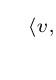
\begin{tikzpicture}[baseline={([yshift=-2ex]current bounding box.north)}, scale=.75][sibling distance=0pt]
		\tikzset{every tree node/.style={align=center,anchor=north}},
		\Tree [.PP\textsubscript{$\langle v,t\rangle$} [.P\\\textit{to}\textsubscript{1}\\{$\langle e,\langle v,t\rangle\rangle$}  ] [.DP\textsubscript{$\langle e\rangle$} [.D\textsubscript{\textsc{[+Ref]}}\\\textit{the}\\{$\langle \langle n,\langle e,t\rangle \rangle ,e \rangle$}  ]  [.{NumP}\textsubscript{$\langle n,\langle e,t\rangle \rangle$} [.\textbf{Num}\\{[\textsc{-PL}]}\\{$\langle \langle n,\langle e,t\rangle \rangle,\langle n,\langle e,t\rangle \rangle \rangle$}  ] [.nP\textsubscript{$\langle n,\langle e,t\rangle \rangle$} [.n\textsubscript{1}\\{$\langle \langle n,\langle e,t\rangle ,\langle n,\langle e,t\rangle \rangle \rangle$}  ] [.root\\{\textit{castle}/\textit{store}\textsubscript{1}/\textit{school}\textsubscript{1}}\\{$\langle n,\langle e,t\rangle \rangle $} ] ] ] ] ] 
		\end{tikzpicture}
	}
\end{exe}
We combine the categorizing head with the \is{countable roots}countable root, which passes up the interpretation of the root. Next, we add in the \isi{number} specification, which restricts the extension of the \is{nouns}noun to singletons. Finally, the type requires that we add the updated Sharvy definite (as in \ref{ex:williams:62}, and then the regular directional \is{prepositions}preposition (as in \ref{ex:williams:65})), resulting in the following derivation:
\begin{exe}
	\ex {[\![n\textsubscript{1} \textit{castle}]\!]\\  
	$= \lambda n.\lambda y. castle(y) \&  \left|\textsc{Atoms}(y)\right| = n  \&  \forall z \in \textsc{Atoms}(y)[ castle(z) ]$}
	\ex {\small{[\![Num\textsc{\textsubscript{[-\textsc{pl}]}} n\textsubscript{1} \textit{castle}]\!] \\ 
	$= \lambda m.\lambda y. castle(y) \&  \left|\textsc{Atoms}(y)\right| = m  \&  \forall z \in \textsc{Atoms}(y)[ castle(z) ] \& m =1 $}}
	\ex {[\![D\textsubscript{[+\textsc{spec}]} Num\textsc{\textsubscript{[-\textsc{pl}]}} n\textsubscript{1} \textit{castle}] ] \\
	$= \iota x.\exists m.[ (castle(x)\&  \left|\textsc{Atoms}(x)\right| = m  \&  \forall z \in \textsc{Atoms}(x)[ castle(z) ]  \\ 
    \& m =1) \& \neg \exists y.[ castle(y) \& \left|\textsc{Atoms}(y)\right| = m \& \forall x' \in \textsc{Atoms}(y)[ castle(y) ] \\ 
    \& m=1 \& x < y $ ] }
	\ex {\label{ex:williams:71} \small{[\![to\textsubscript{1} D\textsubscript{[+\textsc{spec}]} Num\textsc{\textsubscript{[-\textsc{pl}]}} n\textsubscript{1} \textit{castle}]\!]\\ 
	$= \lambda e.$\textsc{Goal}(e)$=\iota x.\exists m.[ (castle(x)\&  \left|\textsc{Atoms}(x)\right| = m \&  
    \forall z \in \textsc{Atoms}(x)[ castle(z) ] \\ 
    \& m =1 ) \& \neg \exists y.[ castle(y) \& \left|\textsc{Atoms}(y)\right| = m \& \forall x' \in \textsc{Atoms}(y)[ castle(y) ] \\
    \&  m=1 \& x < y $ ] }}
\end{exe}

The denotation in \REF{ex:williams:71} gives a set of events whose \textsc{goal} is a \is{uniqueness}unique castle. Some number of atoms is in the extension of \textit{castle} and each of them are also castles, and their cardinality is one (i.e. there is only one of them). Additionally, it asserts that there isn't any other entity (which is a castle that has a number of atoms, which are also castles, and whose cardinality is one) that has the original castle as one of its proper subparts. This is indeed the interpretation we get for the \is{definite noun phrases}strong definite noun phrase.

Compared to a \is{strong definites}strong definite, a weak definite, such as in \REF{ex:williams:3}, differs in at least two ways. First, the denotation of the root is different, resulting in the \is{weak definite articles}weak definite article \REF{ex:williams:66} being merged. Second, these two choices conspire to combine with the \is{incorporation}incorporating adposition. These combinations are required based on the type of the root. 

\begin{exe}
	\ex[]{\label{ex:williams:72}
				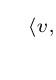
\begin{tikzpicture}[baseline={([yshift=-2ex]current bounding box.north)}, scale=.85][sibling distance=0pt]
				\tikzset{every tree node/.style={align=center,anchor=north}}
				\Tree [.PP\textsubscript{$\langle v,t \rangle$} [.P\\to\textsubscript{2}\\{$\langle \langle k,t\rangle ,\langle v,t\rangle \rangle $}  ] [.DP\textsubscript{$\langle k,t\rangle$} [.D\textsc{[-Ref]}\\\textit{the}\\{$\langle \langle e,t\rangle ,\langle k,t\rangle \rangle$} ]  [.nP\textsubscript{$\langle e,t\rangle $} [.n\textsubscript{2}\\{$\langle \langle e,t\rangle ,\langle e,t\rangle \rangle $} ] [.root\\\textit{store}\textsubscript{2}\\{$\langle e,t\rangle $} ] ] ] ] 
				\end{tikzpicture}
			}
	\ex {[\![n\textsubscript{2} \textit{store}\textsubscript{2}]\!] \\ 
	$= \lambda x. store(x) $}
	\ex {[\![D\textsubscript{[-\textsc{spec}]} n\textsubscript{2} \textit{store}\textsubscript{2}]\!] \\ 
	$= \lambda k.^{\cap}store=k$}
	\ex {[\![\textit{to}\textsubscript{2} D\textsubscript{[-\textsc{spec}]} n\textsubscript{2} \textit{store}\textsubscript{2}]\!] \\
	$= \lambda e. \exists y. \exists k. [^{\cap}store=k\& ^{\cup}k(y) $\textsc{Goal}(e)$=y]$}
\end{exe}

Finally, we take the BIS, as in \REF{ex:williams:4}. Roots that can be bare have the denotation of a \is{kind properties}kind-property (see \ref{ex:williams:58}). This root merges with a categorizing head, which passes up the type and denotation of the root, and then with the \is{incorporation}incorporating \is{prepositions}preposition.

\begin{exe}
	\ex[\label{bis2b}]{ 	
				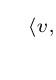
\begin{tikzpicture}[baseline={([yshift=-2ex]current bounding box.north)}, scale=.85][sibling distance=0pt]
				\tikzset{every tree node/.style={align=center,anchor=north}}
				\Tree [.PP\textsubscript{$\langle v,t \rangle $}  [.P\\\textit{to}\\{$\langle \langle k,t\rangle ,\langle v,t\rangle \rangle $}   ] [.nP\textsubscript{$\langle k,t\rangle $}  [.n\textsubscript{3}\\{$\langle \langle k,t\rangle ,\langle k,t \rangle \rangle $} ] [.root\\\textit{school}\textsubscript{2}\\{$\langle k,t\rangle $} ] ] ]
				\end{tikzpicture}
			}
	\ex {[\![n\textsubscript{3} \textit{store}\textsubscript{2}]\!] \\ 
$= \lambda k. school(k) $}
	\ex {[\![\textit{to}\textsubscript{2} D\textsubscript{[-\textsc{spec}]} n\textsubscript{2} \textit{school}\textsubscript{2}]\!] \\
	$= \lambda e. \exists y. \exists k.[school(k)\& ^{\cup}k(y) \& $\textsc{Goal}(e)$=y]$}
\end{exe}

The derivation for the BIS reflects their similarity with weak definites. More specifically, both derivations lack a {Num} projection, and combine with the incorporating adposition. 

\section{Conclusion}\label{sec:williams:6}

I have argued that weak definites and \isi{bare singulars} mean similar things (both are \is{number neutrality}number neutral), and share comparable \is{morphosyntax}morphosyntactic structure (both lack a {Num} projection, and merge with an incorporating adposition). Roots that participate in weak nominal constructions divide into two lexical classes; one participates in weak definite constructions and the other participates in BIS constructions. These two classes are distinct, with no single lexical item can participate in both weak definite and BIS constructions. Lexical items from these classes are \is{semantic root ambiguity}semantically type ambiguous at the root level, with two denotations each. This semantic ambiguity affects whether the root can appear in particular syntactic configurations (e.g. whether it requires an overt strong \is{determiners}determiner to be merged).   

Interpretive differences between strong and weak nominals correspond to differences at two syntactic positions: first, at the root-level, semantic type ambiguity determines which interpretation(s) is/are possible, and second, at the determiner-level, the semantic type of the root conditions which of two versions of the definite determiner will be chosen. Using these two ingredients, this account explains why weak definites and \isi{bare singulars} receive \is{number neutrality}number neutral interpretations, while simultaneously explaining their lexical idio\-syncrasies.\is{weak definites|)}\is{morphosemantics|)}

\section*{Acknowledgements}
Special thanks to Ruth Kramer and the students in her Seminar on the Syntax of Number (NYU, Spring 2015); to Curt Anderson, David Beaver, Hagen Blix, Dylan Bumford, Lucas Champollion, Simon Charlow,  Chris Collins, Masha Esipova, Paloma Jereti{\v c}, Maria Kouneli, Marcin Morzycki, Alan Munn, Neil Myler, Rob Pasternak, Sarah Phillips, and Anna Szabolcsi for advice, skepticism, criticism, proofreading, and/or encouragement; to the members of Rutgers' SURGE and New York University's MorphBeer; the audiences, organizers, and reviewers for Definiteness across Languages; and finally, to attendees of SYNC 2013 and SWAMP 2012 for comments on much earlier versions of this work. \is{bare institutional singulars|)}

\section*{Abbreviations}
\begin{tabular}{ll}
	\textsc{bis} & Bare institutional singular \\
	\textsc{num} & Number \\
	\textsc{pl} & Plural \\
	\textsc{ref} & Referential \\
\end{tabular}

{\sloppy
\printbibliography[heading=subbibliography,notkeyword=this]
}
\end{document}
